\documentclass[11pt,a4paper]{article}
\usepackage[margin=2.2cm]{geometry}
\usepackage[pdftex]{graphicx}
\usepackage{styles}
\usepackage{url} 
\usepackage[bookmarks, colorlinks=false, pdfborder={0 0 0}, pdftitle={Formal verification of programs with pointers}, pdfauthor={Oualid CHABANE}]{hyperref} 
\usepackage{minted}
\usepackage{tikz}
\usepackage{colortbl}
\usepackage{hyperref}
\usepackage{textcomp}
\usepackage{amssymb}
\usepackage{titlesec}
\usepackage{parskip}
\usepackage{enumitem}
\usepackage{parskip}
\usepackage{amsmath}
\usepackage{xcolor}
\usepackage{titlesec}
\usepackage{hyperref}
\usepackage{biblatex}
\usetikzlibrary{matrix, arrows.meta, positioning, fit}
\usetikzlibrary{calc}
\usetikzlibrary{decorations.pathreplacing}
\addbibresource{bibliography.bib}
% Indent subsections by 1em
\titlespacing*{\subsection}{1em}{1ex plus .2ex minus .2ex}{0.5ex}

% (Optional) Further indent subsubsections
\titlespacing*{\subsubsection}{2em}{1ex plus .2ex minus .2ex}{0.5ex}

\setlength{\parindent}{1.5em} % Re-enable paragraph indentation

% Reduce line spacing
\linespread{1.0}


\begin{document}
\begin{titlepage}

\begin{center}

\textup{\small {\bf Summer Internship Project} \\ Report}\\[0.3in]

% Title
\Large \textbf {\scol{\bf Formal verification of programs with pointers }}\\[0.7in]


       

% Submitted by
\normalsize Submitted by \\[0.2in]
\scol{\textbf{Oualid CHABANE}}\\
Third year of bachelor's double degree in \\ Computer Science, Magistère d'informatique track.\\
Faculty of sciences of Orsay, university of Paris-Saclay.

\vspace{.2in}
Under the guidance of\\[0.2in]
\scol{\textbf{Arnaud Goulfouse}}\\
\scol{\textbf{Paul Patault}}\\
\scol{\textbf{Jean-Christophe Filliâtre}}\\

\vspace{.3in}

% Bottom of the page
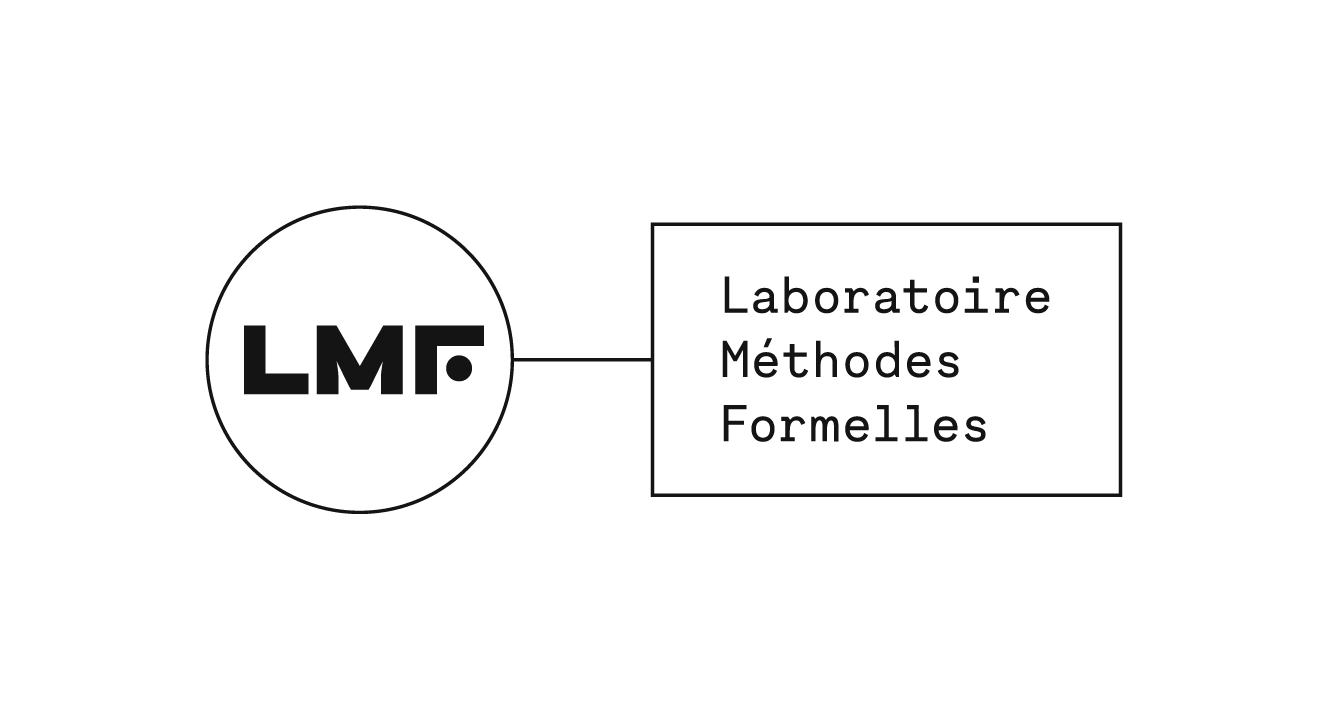
\includegraphics[width=0.5\textwidth]{lmf.png}\\[0.1in]
\Large{Department of Formal methods}\\
\normalsize
\textsc{ The Laboratoire Méthodes Formelles (LMF). }\\
4, avenue des Sciences, 91190 Gif-sur-Yvette \\
\vspace{0.2cm}
Summer Internship 2025

\end{center}

\end{titlepage}


\pagenumbering{roman}
\tableofcontents

\newpage
\pagenumbering{arabic} 


\newcommand{\rust}{\textsc{Rust}}
\newcommand{\creusot}{\textsc{Creusot}}
\newcommand{\why}{\textsc{Why3}}

\section{Introduction}

\subsection{\scol{The Laboratoire Méthodes Formelles (LMF)}}
 LMF is a joint research center of Paris-Saclay University, CNRS, ENS Paris-Saclay, Inria, and CentraleSupélec. It's divided in multiple departments interested in various topics such as type systems, quantum computing and topology. My research project took place within \scol{Toccata's team} of the formal methods department. I worked on verification of programs with pointers under the supervision of Jean-Christophe Filliâtre, Arnaud Golfouse and Paul Patault.

There are multiple verification tools widely used and developed at the LMF research center. Among these tools, we find \creusot{} and \why{}.

\subsection{\scol{\creusot{} tool}}
\subsubsection{\scol{Introduction}}
\creusot{}~\cite{jh} is a formal verification tool designed for \rust{} code. It guarantees safety by detecting compile-time errors, runtime panics, and integer overflows, while also ensuring that the code respects its formal specification.

\creusot{} operates on top of \why{} indirectly by translating \rust{} code into an intermediate verification language known as \textsc{Coma}. It facilitates the verification, and it also gives \creusot{} access to the full access to \why{}'s backend.

In \autoref{fig:sum-example} is a simple example of \creusot{} code that verifies the correctness of the \texttt{sum\_first\_n} function.

\begin{figure}[tp]
\centering
\begin{minipage}{0.95\linewidth}
\begin{minted}[linenos, fontsize=\footnotesize, bgcolor=gray!5]{rust}
extern crate creusot_contracts;
use creusot_contracts::*;

#[requires(n@ * (n@ + 1) / 2 < u32::MAX@)]
#[ensures(result@ == n@ * (n@ + 1) / 2)]
pub fn sum_first_n(n: u32) -> u32 {
    let mut sum = 0;
    #[invariant(sum@ * 2 == produced.len() * (produced.len() + 1))]
    for i in 1..=n {
        sum += i;
    }
    sum
}
\end{minted}
\caption{\creusot{} verification example: sum of first \texttt{n} natural numbers}
\label{fig:sum-example}
\end{minipage}
\end{figure}

\textbf{Explanation}: 

The function \texttt{sum\_first\_n} in \autoref{fig:sum-example} computes the sum of the first \texttt{n} natural numbers. The special comments denoted with \texttt{\#[...]} represent its specification:
\begin{itemize}
\item \textbf{Precondition:} It asserts that the sum of the first \texttt{n} natural numbers where \texttt{n} is provided as a parameter, does not overflow the capacity of the result type. This ensures that the final sum, which will be stored in the return variable will not exceed the capacity of the return type. The operator \texttt{@} converts machine integers into mathematical integers, which are unbounded, allowing us to use arithmetic theory.
\item \textbf{Postcondition:} It states that the returned result is equal to the expected mathematical value: \texttt{n * (n + 1) / 2}.
\item \textbf{Loop invariant:} The expression \texttt{produced.len()} corresponds to the number of iterations performed so far. It effectively can play the role of the loop index by applying a transformation. The reason we cannot refer directly to the loop index is due to scoping limitations.
\end{itemize}
\subsubsection{\scol{Ghost code in \creusot{}}}
\rust{}'s ownership and borrowing principles make it difficult to use pointers in proofs, where the need for a notion of ghost code in such a language. Ghost code~\cite{jcfand} allows us to perform proofs that are not possible using only raw code and the logical world, especially when dealing with existential quantification, if we know how to construct the value we are seeking for the existential quantifier.

Recently, ghost code has been introduced in \creusot{}. Ghost code is separate from normal code via syntax and typing. Therefore, it can be safely erased at compile time, allowing only the original code to be executed. This results in more expressive proof verification. In \autoref{fig:ghost-example} are some examples of how to write ghost code in \creusot{}.

\hypertarget{ghostcode}{}
\begin{figure}[tp]
  \centering
  \begin{minted}[linenos, fontsize=\footnotesize, bgcolor=gray!5]{rust}
let mut g = ghost!(50);
ghost! {
    *g *= 2;
};
proof_assert!(g@ == 100);
  \end{minted}
  \caption{An example of ghost state manipulation in \creusot{}.}
  \label{fig:ghost-example}
\end{figure}

\section{State of art}

\subsection{\scol{Reynolds' separation logic}}
Reynolds~\cite{reynolds} introduces a new concept in formal program verification, \emph{Separation Logic} is an extension of Hoare's Logic that facilitates automatic proofs on low-level imperative programs that use shared mutable data structures, by reasoning about disjoint parts of the heap. It greatly simplifies the formalization and verification of many problems that are otherwise difficult to handle using traditional Hoare's Logic, such as aliasing, memory management, and concurrency.
\\

Reynolds is particularly interested in the \hyperlink{reversal}{\texttt{in\_place\_reversal}$\dagger$} algorithm. He frequently discusses it in this research paper, as it is a very interesting algorithm for exploring formal proofs on mutable data structures with pointers.
\\

To prove properties of algorithms on data structures, it's usually not enough to rely only on the program's representation. We often build a logical model of the data and connect it to the program state using predicates. For instance, the intuitive logical modeling of lists are sequences, therefore we can write the following predicate to represent a list:


\begin{align*}
\texttt{list}\ \epsilon\ \texttt{i} &\overset{\text{def}}{=}\ \texttt{i = nil} \\
\texttt{list}\ (a.\alpha)\ \texttt{i} &\overset{\text{def}}{=}\ \exists\ \texttt{j},\ \texttt{list}\ \alpha\ \texttt{j} \land\ \texttt{i} \hookrightarrow \texttt{a, j}
\end{align*}


where \texttt{i $\hookrightarrow$ a} means "\texttt{i} points to \texttt{a}"\\.
The predicate \texttt{list} allows us to link the code pointer \texttt{i} into it's corresponding sequence $\alpha$.\\
If we extend the proof to lassos, it would be better to define a list in a more general way, so that a list is identified by a pair of pointers: the first pointer represents the head of the sub-list, and the second pointer represents the tail of the sub-list. This way, we can separate the lasso into its two main parts, the cycle and the entry list.

One of key uses of separation logic can be seen when trying to use \hyperlink{reversal}{\texttt{in\_place\_reversal}$\dagger$} on shared data structures, in this context, given the following precondition for in-place reversal: \texttt{list p $\alpha$}, the post-condition \texttt{list p }$\overline{\alpha}$ is not sufficient to ensure the correctness of the algorithm. Consider the example in \autoref{fig:shared-lists}.

\begin{figure}[tp]
\centering
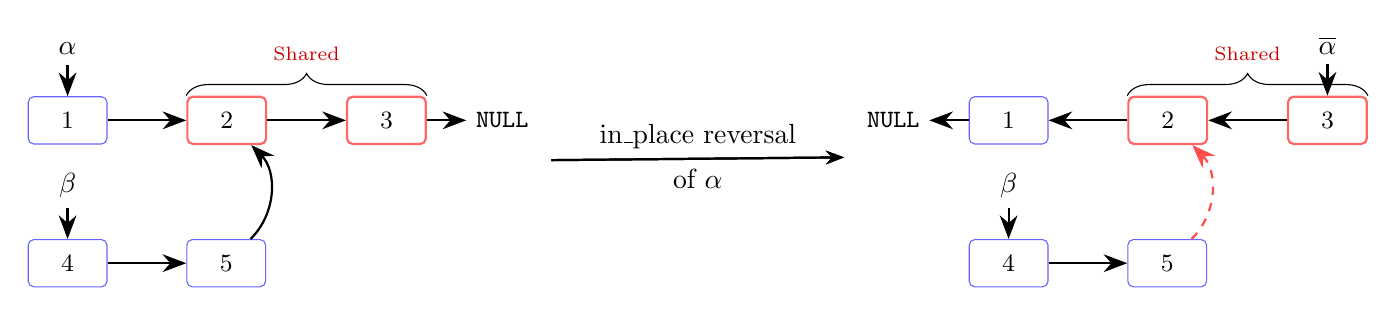
\begin{tikzpicture}[node distance=1cm and 1cm, 
    box/.style={
        rectangle, draw, minimum width=1cm, minimum height=0.6cm, rounded corners=2pt,
        font=\small, text centered
    },
    normal/.style={draw=blue!60},
    shared/.style={draw=red!60, thick},
    arrow/.style={-{Stealth[length=3mm]}, thick},
    label/.style={font=\bfseries}
]

% First diagram as a scope
\begin{scope}[local bounding box=first]
    % List A nodes
    \node[box, normal] (a1) {1};
    \node[box, shared, right=of a1] (shared3) {2};
    \node[box, shared, right=of shared3] (shared4) {3};

    % List B nodes
    \node[box, normal, below=1.2cm of a1] (b6) {4};
    \node[box, normal, right=of b6] (b7) {5};

    % List head labels
    \node[label, above=0.4cm of a1] (listA) {$\alpha$};
    \node[label, above=0.4cm of b6] (listB) {$\beta$};

    % Arrows for List A
    \draw[arrow] (listA) -- (a1);
    \draw[arrow] (a1) -- (shared3);
    \draw[arrow] (shared3) -- (shared4);

    % Arrows for List B
    \draw[arrow] (listB) -- (b6);
    \draw[arrow] (b6) -- (b7);
    \draw[arrow, bend right=45] (b7) to (shared3);

    % Null pointer
    \node[right=0.5cm of shared4, font=\small\ttfamily] (null1) {NULL};
    \draw[arrow] (shared4) -- (null1);

    % Brace for shared nodes
    \draw [decorate, decoration={brace, amplitude=8pt}]
      (shared3.north west) -- (shared4.north east) 
      node[midway, yshift=15pt, font=\scriptsize\color{red!80!black}] {Shared};
\end{scope}

% Second diagram as a scope, shifted right by 8cm (adjust as needed)
\begin{scope}[xshift=16cm, local bounding box=second]
    % List A nodes (right to left)
    \node[box, shared] (shared4b) {3};
    \node[box, shared, left=of shared4b] (shared3b) {2};
    \node[box, normal, left=of shared3b] (a1b) {1};
    
    % List B nodes
    \node[box, normal, below=1.2cm of a1b] (b6b) {4};
    \node[box, normal, right=of b6b] (b7b) {5};
    
    % List head labels
    \node[label, above=0.4cm of shared4b] (listAb) {$\overline{\alpha}$};
    \node[label, above=0.4cm of b6b] (listBb) {$\beta$};
    
    % Arrows for List A (reversed)
    \draw[arrow] (listAb) -- (shared4b);
    \draw[arrow] (shared3b) -- (a1b);
    \draw[arrow] (shared4b) -- (shared3b);
    
    % Arrows for List B
    \draw[arrow] (listBb) -- (b6b);
    \draw[arrow] (b6b) -- (b7b);
    \draw[arrow, dashed, color=red!70, bend right=45] (b7b) to (shared3b);
    
    % Null pointer at the end of the list
    \node[left=0.5cm of a1b, font=\small\ttfamily] (null1b) {NULL};
    \draw[arrow] (a1b) -- (null1b);
    
    % Brace for shared part
    \draw [decorate, decoration={brace, amplitude=8pt}]
      (shared3b.north west) -- (shared4b.north east)
      node[midway, yshift=15pt, font=\scriptsize\color{red!80!black}] {Shared};
\end{scope}
% Arrow between diagrams
\draw[->, thick, >=Stealth, shorten >=5pt, shorten <=5pt] 
  (first.east) -- node[above] {in\_place reversal} (second.west);
\draw[->, thick, >=Stealth, shorten >=5pt, shorten <=5pt] 
  (first.east) -- node[below] {of $\alpha$} (second.west);

\end{tikzpicture}

\caption{\texttt{in\_place reversal} on shared lists}
\label{fig:shared-lists}
\end{figure}

So we need to provide a stronger precondition that prevents such cases. One possible way is:
\[
\texttt{list\ p\ }\alpha \ \land\ \forall\,\texttt{x},\, \alpha'.\ \texttt{list\ x\ } \alpha' \rightarrow \texttt{conflicting}(\texttt{x},\ \alpha',\ \texttt{p},\ \alpha) \rightarrow \texttt{x} = \texttt{nil}
\]

where \texttt{conflicting: Pointer -> Pointer -> bool} is a predicate that returns \texttt{True} if the two provided lists share any nodes. It is defined as follows:
\begin{align*}
\texttt{conflicting}\ \texttt{ nil } \texttt{p'}\ &\overset{\text{def}}{=} \texttt{false} \\
\texttt{conflicting}\ \texttt{ p } \texttt{nil}\ &\overset{\text{def}}{=} \texttt{false} \\
\texttt{conflicting}\ \texttt{p}\ \texttt{p'}\  &\overset{\text{def}}{=} \texttt{p} = \texttt{p'} \lor {} \nonumber \\
&\quad \exists \texttt{a, q, p'} \hookrightarrow \texttt{a, q } \land \texttt{ conflicting}\ \texttt{ p }\  \texttt{q}\ \lor {} \nonumber \\
&\quad \exists \texttt{a, q, p } \hookrightarrow \texttt{a, q } \land \texttt{ conflicting}\ \texttt{ q }\ \texttt{p'}\ 
\end{align*}

In \textsc{Creusot}, we will need to provide the sequences associated with the pointers to obtain the permissions required to access their successors.\\
We can clearly notice that the precondition, but also the invariant, and the post-condition become extremely complicated. This is where separation logic proves invaluable. By leveraging heap separation, the specifications become significantly clearer and simpler.\\
\begin{align*}
    \texttt{list $\epsilon$ p} & \overset{def}{=} \texttt{ p = nil}\\
    \texttt{list $a.\alpha$ p} & \overset{def}{=} \texttt{p $\hookrightarrow$ a, p' *  list $\alpha$ p'}
\end{align*}

Although \creusot{} does not support Separation Logic, its principles can be emulated through the use of the \rust{} type system and ghost code.
The latter can be used to carry over separation logic principles that are implicitly guaranteed by the \rust{} type system into the logical world. To be more precise, let us consider the interface of \texttt{PtrOwn<T>::disjoint\_lemma} as an illustrative example.

\begin{figure}[tp]
\centering
\begin{minipage}{0.9\linewidth}
\begin{minted}[linenos, fontsize=\footnotesize, bgcolor=gray!5]{rust}
/// Ensures two PtrOwns reference different memory locations
#[ghost]
#[ensures(own1.ptr().addr_logic() != own2.ptr().addr_logic())]
#[ensures(*own1 == ^own1)]
pub fn disjoint_lemma(own1: &mut PtrOwn<T>, own2: &PtrOwn<T>)
\end{minted}
\caption{\texttt{PtrOwn<T>::disjoint\_lemma} interface}
\end{minipage}
\end{figure}

This lemma is admitted as an axiom in \creusot{}, and what it does is verify that the two permissions correspond to two distinct pointers on the heap.
If this lemma was logical, it would not hold, because we quantify universally over \texttt{own1} and \texttt{own2} and we can't guarantee separation in \textsc{Creusot}'s  logic. Therefore, one could be equal to the other, and the first post-condition would not be satisfied.
However, if we admit it as a ghost lemma, the \rust{} type system, within the context of ghost code prohibits having a mutable borrow and an immutable borrow to the same value.
Therefore, \texttt{own1} and \texttt{own2} are necessarily distinct, and the validity of the axiom follows (the second post-condition is not essential for conveying the idea).

There are, however, more specialized tools designed specifically for reasoning with Separation Logic. One such tool is \textsc{Prusti}, a \rust{} verifier that supports Separation Logic. It is built on top of \textsc{Viper} which is built on top of \textsc{Boogie}, an intermediate verification language (IVL) developed by Microsoft Research, and is widely used in the field of formal verification. The \autoref{fig:verification-diagram} clarifies the relationships between these languages and their connection to Separation Logic.

\begin{figure}[tp]
\centering
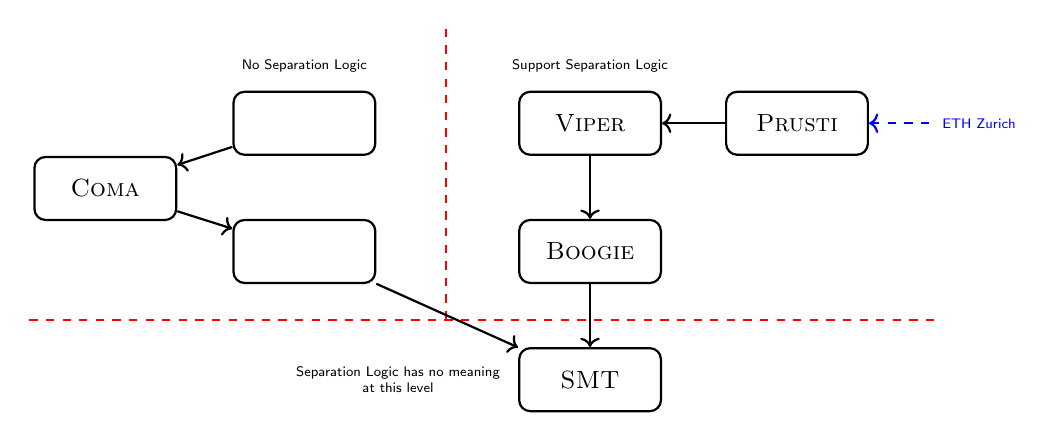
\begin{tikzpicture}[
  node distance=0.8cm and 1.8cm,
  every node/.style={font=\sffamily\small},
  box/.style={draw, rectangle, rounded corners, minimum width=1.8cm, minimum height=0.8cm, align=center},
  ->, thick
]
% Nodes
\node[box] (creusot) {\creusot{}};
\node[box, right=of creusot] (viper) {\textsc{Viper}};
\node[box, below=of viper] (boogie) {\textsc{Boogie}};
\node[box, left=of boogie] (why3) {\why{}};
\node[box, below left=0cm and 0.7cm of creusot] (coma) {\textsc{Coma}};
\node[box, below=of boogie] (smt) {\textsc{SMT}};
\node[box, right=0.8cm of viper] (delphi) {\textsc{Prusti}};

% Arrows
\draw[-, dashed, red, line width=0.8pt] 
  (1.8,1.2) -- (1.8,-2.5);

\draw[-, dashed, red, line width=0.8pt] 
  (8,-2.5) -- (-3.5,-2.5);
  
\draw (creusot) -- (coma);
\draw (coma) -- (why3);
\draw (viper) -- (boogie);
\draw (why3) -- (smt);
\draw (boogie) -- (smt);
\draw (delphi) -- (viper);




\draw[<-, dashed, blue] (delphi.east) -- ++(0.8,0) node[right, font=\tiny\sffamily, blue] {ETH Zurich};

% Add explanatory labels
\node[above=0.1cm of creusot, align=center, font=\tiny\sffamily] (leftlabel) 
  {No Separation Logic};
\node[above=0.1cm of viper, align=center, font=\tiny\sffamily] (rightlabel) 
  {Support Separation Logic};
\node[left=0.1cm of smt, align=center, font=\tiny\sffamily] (rightlabel) 
  {Separation Logic has no meaning\\ at this level};
\end{tikzpicture}
\caption{Illustration of the relationship between verification tools and intermediate languages.}
\label{fig:verification-diagram}
\end{figure}

\subsection{\scol{Different ways of implementing the problem}}
The list reversal problem has already been proven in two different ways in \creusot{}, but both methods have certain limitations:

\begin{itemize}
\item \hypertarget{BOXmeth}{\textbf{\textsc{BOX} method}}: This approach models lists using \rust{} \texttt{Box} type. However, it imposes strong restrictions on the memory model by prohibiting any form of sharing or aliasing, since \texttt{Box} does not support multiple references to the same memory location. As a result, the specification is simple and the proof goes through easily.
\item \hypertarget{MEMmodel}{\textbf{Memory model method}}: This approach relies on modular reasoning over the memory. In other words, it involves passing an object that models the entire memory as a parameter to each method to be verified. As a result, verification requires reasoning about the complete memory state. This can quickly lead to complex proofs even for simple algorithms. For example, suppose we have two disjoint lists in the heap, each verified using a \texttt{list} predicate. If we reverse one of them, the \texttt{list} predicate on the other is not preserved automatically, and we must explicitly include it in the proof. This makes the verification process tedious. This is where separation logic becomes useful, and the solution we propose implicitly uses its principles, thanks to \rust{} type system.
\end{itemize}

\section{Problem definition and proposed solution}
\subsection{\scol{Problem definition}}
Formal verification of mutable data structures with pointers is one of the most challenging aspects of formal methods. The in-place list reversal algorithm is a canonical example of this challenge, as it can easily lead to memory leaks, dangling pointers, or logical errors.\\
The core problem is that, for a given list implementation in \rust{} using raw pointers, we need to formally verify the correctness of an in-place reversal algorithm. Not only that, but also the preservation of memory safety and the proper handling of shared lists. The rust code that we have proposed is in \autoref{fig:reversalinp}

\begin{figure}[tp]
    \begin{minted}[breaklines=true]{rust}
    pub fn reverse_in_place(mut p: RawPtr<Self>) -> RawPtr<Self> {
        let mut q: *const Node<T> = ptr::null();
        while !p.is_null() {
            let p2 = unsafe { &mut *p };
            let next = p2.next;
            p2.next = q;
            q = p;
            p = next;
        }
        q
    }
    \end{minted}
\caption{Rust code of \texttt{in\_place\_reversal}.}
\label{fig:reversalinp}
\end{figure}


\subsection{\scol{Proposed solution}}
\subsubsection{\scol{\texttt{PtrOwn} and \texttt{RawPtr}}} Used by \creusot{} to manipulate pointers in proofs. \texttt{PtrOwn} models ownership of memory cells in the ghost world and can be used in parallel with \texttt{RawPtr}, which represents the corresponding address of the cell represented by \texttt{PtrOwn}. The internal representation of \texttt{PtrOwn} is shown in \autoref{fig:ptrown-structure}.

\begin{figure}[tp]
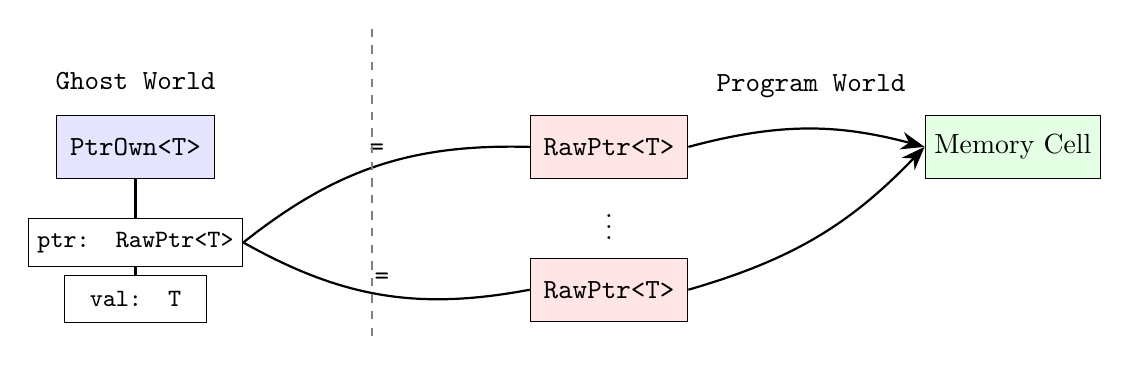
\begin{tikzpicture}[
    node distance=1cm,
    box/.style={rectangle, draw, minimum width=2cm, minimum height=0.8cm, text centered},
    field/.style={rectangle, draw, minimum width=1.8cm, minimum height=0.6cm, text centered, font=\small},
    arrow/.style={-{Stealth[length=3mm]}, thick}
]

% PtrOwn structure
\node[box, fill=blue!10] (ptrOwn) at (0,0) {\texttt{PtrOwn<T>}};

% Fields of PtrOwn
\node[field, below=0.5cm of ptrOwn] (ptrField) {\texttt{ptr: RawPtr<T>}};
\node[field, below=0.1cm of ptrField] (valField) {\texttt{val: T}};

% External RawPtr box
\node[box, fill=red!10, right=4cm of ptrOwn] (rawPtrBox) {\texttt{RawPtr<T>}};
\node[box, fill=red!10, below=1cm of rawPtrBox] (rawPtrBox2) {\texttt{RawPtr<T>}};
\node at ($(rawPtrBox)!0.5!(rawPtrBox2)$) {\vdots};


% Memory cell that RawPtr points to
\node[box, fill=green!10, right=3cm of rawPtrBox] (memoryCell) {Memory Cell};

% Arrows
% Beautiful curved arrows
\draw[thick, bend left=20] (ptrField.east) to node[midway, above] {\texttt{=}} (rawPtrBox.west);
\draw[thick, bend right=20] (ptrField.east) to  node[midway, above] {\texttt{=}} (rawPtrBox2.west);
\draw[arrow, bend left=15] (rawPtrBox.east) to (memoryCell.west);
\draw[arrow, bend right=15] (rawPtrBox2.east) to (memoryCell.west);

% Labels
\node[above=0.2cm of ptrOwn] {\texttt{Ghost World}};
\node at ($(rawPtrBox)!0.5!(memoryCell)$) [above=0.5cm] {\texttt{Program World}};


% Connecting lines for structure
\draw[thick] (ptrOwn.south) -- (ptrField.north);
\draw[thick] (ptrField.south) -- (valField.north);
% Vertical separator line
\draw[gray, thick, dashed] ($(ptrOwn.east)!0.5!(rawPtrBox.west) + (0,1.5)$) -- ($(ptrOwn.east)!0.5!(rawPtrBox.west) + (0,-2.5)$);


\end{tikzpicture}
\caption{Internal structure of \texttt{PtrOwn<T>}.}
\label{fig:ptrown-structure}
\end{figure}

Our solution relies on the use of linear algebraic types in \creusot{}, specifically, \texttt{PtrOwn} and \texttt{RawPtr}. This allows us to prove the correctness of in-place reversal even in the presence of shared data structures, making it better than the \hyperlink{BOXmeth}{BOX method$\dagger$}. Moreover, it also outperforms the \hyperlink{MEMmodel}{memory model$\dagger$} approach, our method requires to reason locally on memory. In other words, we only need to verify the parts of the heap we are manipulating, without having to reason about independent regions. This provides a form of separation logic, implicitly enforced by the rust type system.\\
In the following we will present our solutions in steps.\\
\subsubsection{\scol{Data Structure}}
The list type is represented by \texttt{RawPtr<Node<T>>} where \texttt{Node<T>} is defined like the following:
\begin{minted}[linenos, fontsize=\footnotesize, bgcolor=gray!5]{rust}
struct Node<T> {
    elem: T,
    pub next: RawPtr<Node<T>>,
}
\end{minted}

\subsubsection{\scol{Predicates}}
\begin{itemize}
    \item  \hyperlink{list}{\textbf{The \texttt{list} Predicate}
      $\dagger$}\\
        We defined a predicate \texttt{list} that takes a pointer of type \texttt{RawPtr} and the abstract ghost sequence of permission \texttt{PtrOwn} that represents the list algebraically \texttt{seq}. It checks recursively that the pointers inside the permissions in the sequence correspond to the pointers in the program world, and that the list ends with \texttt{nil}.\\
    \begin{minted}{rust}
    #[predicate]
    #[variant(perm_seq.len())]
    fn list(l: RawPtr<Self>, perm_seq: Seq<PtrOwn<Node<T>>>) -> bool {
        if l.is_null_logic() {
            perm_seq.len() == 0
        } else {
             if perm_seq.len() > 0 {
                let ptr = perm_seq[0].ptr();
                l == ptr && Self::list(perm_seq[0].val().next, perm_seq.tail())
            } else {
                false
            }
        }
    }
    \end{minted}
    
  \begin{figure}[tp]
    \centering
    % Option 1: Single tikzpicture with both diagrams
    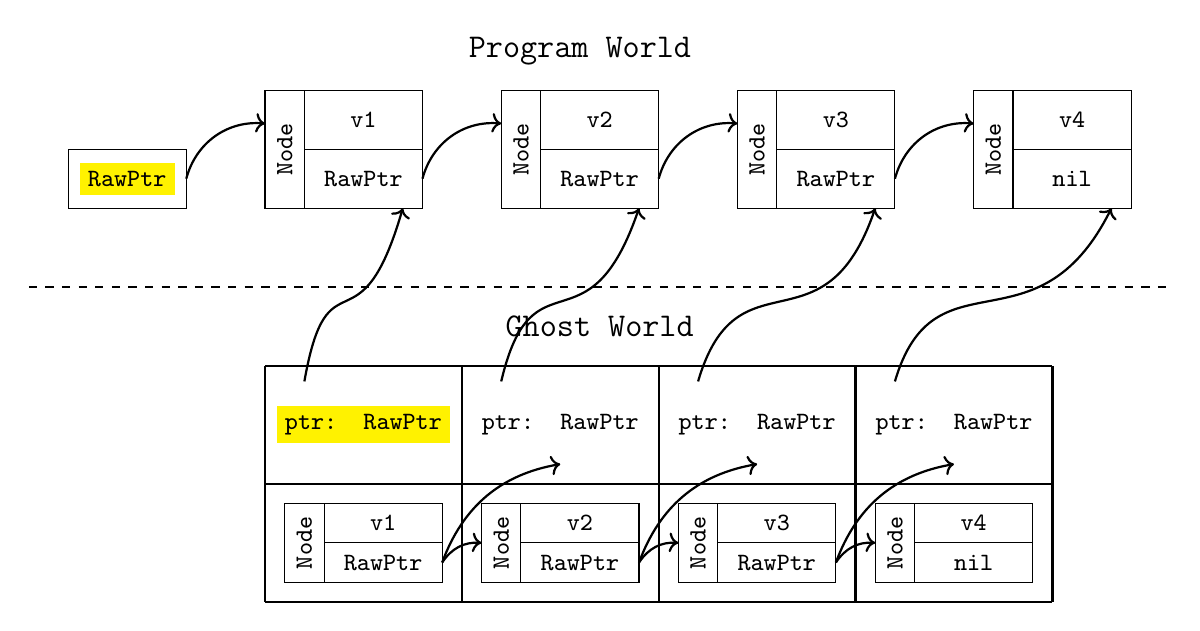
\begin{tikzpicture}
    % Program World
    \node[font=\large\bfseries] at (4,16.5) {\texttt{Program World}};
    
    \draw (-2.5,14.5) rectangle (-1,15.25);
    \node[font=\small] at (-1.75,14.875) {\texttt{\colorbox{yellow}{RawPtr}}};
    \draw[->, thick, bend left=40] (-1,14.875) to (0,15.575);
    
    % First Node
    \draw (0,14.5) rectangle (0.5,16);
    \draw (0.5,14.5) rectangle (2,15.25);
    \draw (0.5,15.25) rectangle (2,16);
    \node[rotate=90, font=\small] at (0.25,15.25) {\texttt{Node}};
    \node[font=\small] at (1.25,15.625) {\texttt{v1}};
    \node[font=\small] at (1.25,14.875) {\texttt{RawPtr}};
    
    % Arrow to second node
    \draw[->, thick, bend left=40] (2,14.875) to (3,15.575);
    
    % Second Node
    \draw (3,14.5) rectangle (3.5,16);
    \draw (3.5,14.5) rectangle (5,15.25);
    \draw (3.5,15.25) rectangle (5,16);
    \node[rotate=90, font=\small] at (3.25,15.25) {\texttt{Node}};
    \node[font=\small] at (4.25,15.625) {\texttt{v2}};
    \node[font=\small] at (4.25,14.875) {\texttt{RawPtr}};
    
    % Arrow to third node
    \draw[->, thick, bend left=40] (5,14.875) to (6,15.575);
    
    % Third Node
    \draw (6,14.5) rectangle (6.5,16);
    \draw (6.5,14.5) rectangle (8,15.25);
    \draw (6.5,15.25) rectangle (8,16);
    \node[rotate=90, font=\small] at (6.25,15.25) {\texttt{Node}};
    \node[font=\small] at (7.25,15.625) {\texttt{v3}};
    \node[font=\small] at (7.25,14.875) {\texttt{RawPtr}};
    
    % Arrow to fourth node
    \draw[->, thick, bend left=40] (8,14.875) to (9,15.575);
    
    % Fourth Node
    \draw (9,14.5) rectangle (9.5,16);
    \draw (9.5,14.5) rectangle (11,15.25);
    \draw (9.5,15.25) rectangle (11,16);
    \node[rotate=90, font=\small] at (9.25,15.25) {\texttt{Node}};
    \node[font=\small] at (10.25,15.625) {\texttt{v4}};
    \node[font=\small] at (10.25,14.875) {\texttt{nil}};
    
    % Dashed divider line
    \draw[dashed, thick] (-3,13.5) -- (11.5,13.5);
    
    % Ghost World
    \node[font=\large\bfseries] at (4.25,13) {\texttt{Ghost World}};
    
    % Manual grid lines for 4 columns
    % Vertical lines
    \draw[black, thick] (0,9.5) -- (0,12.5);
    \draw[black, thick] (2.5,9.5) -- (2.5,12.5);
    \draw[black, thick] (5,9.5) -- (5,12.5);
    \draw[black, thick] (7.5,9.5) -- (7.5,12.5);
    \draw[black, thick] (10,9.5) -- (10,12.5);
    
    % Horizontal lines
    \draw[black, thick] (0,9.5) -- (10,9.5);     % Bottom
    \draw[black, thick] (0,11) -- (10,11);       % Middle
    \draw[black, thick] (0,12.5) -- (10,12.5);   % Top
    
    % Column 1
    \node[font=\small] at (1.25,11.75) {\texttt{\colorbox{yellow}{ptr: RawPtr}}};
    \draw (0.25,9.75) rectangle (0.75,10.75);
    \draw (0.75,9.75) rectangle (2.25,10.25);
    \draw (0.75,10.25) rectangle (2.25,10.75);
    \node[rotate=90, font=\small] at (0.5,10.25) {\texttt{Node}};
    \node[font=\small] at (1.5,10.5) {\texttt{v1}};
    \node[font=\small] at (1.5,10) {\texttt{RawPtr}};
    
    % Column 2
    \node[font=\small] at (3.75,11.75) {\texttt{ptr: RawPtr}};
    \draw (2.75,9.75) rectangle (3.25,10.75);
    \draw (3.25,9.75) rectangle (4.75,10.25);
    \draw (3.25,10.25) rectangle (4.75,10.75);
    \node[rotate=90, font=\small] at (3,10.25) {\texttt{Node}};
    \node[font=\small] at (4,10.5) {\texttt{v2}};
    \node[font=\small] at (4,10) {\texttt{RawPtr}};
    
    % Column 3
    \node[font=\small] at (6.25,11.75) {\texttt{ptr: RawPtr}};
    \draw (5.25,9.75) rectangle (5.75,10.75);
    \draw (5.75,9.75) rectangle (7.25,10.25);
    \draw (5.75,10.25) rectangle (7.25,10.75);
    \node[rotate=90, font=\small] at (5.5,10.25) {\texttt{Node}};
    \node[font=\small] at (6.5,10.5) {\texttt{v3}};
    \node[font=\small] at (6.5,10) {\texttt{RawPtr}};
    
    % Column 4
    \node[font=\small] at (8.75,11.75) {\texttt{ptr: RawPtr}};
    \draw (7.75,9.75) rectangle (8.25,10.75);
    \draw (8.25,9.75) rectangle (9.75,10.25);
    \draw (8.25,10.25) rectangle (9.75,10.75);
    \node[rotate=90, font=\small] at (8,10.25) {\texttt{Node}};
    \node[font=\small] at (9,10.5) {\texttt{v4}};
    \node[font=\small] at (9,10) {\texttt{nil}};
    
    % Cross-reference arrows from Ghost World to Program World
    \draw[->, thick] (0.5,12.3) .. controls (0.8,14) and (1.2,12.6) .. (1.75,14.5);
    \draw[->, thick] (3,12.3) .. controls (3.4,14) and (4.1,12.6) .. (4.75,14.5);
    \draw[->, thick] (5.5,12.3) .. controls (6,14) and (7.1,12.6) .. (7.75,14.5);
    \draw[->, thick] (8,12.3) .. controls (8.5,14) and (9.8,12.6) .. (10.75,14.5);
    
    % Internal Ghost World arrows
    \draw[->, thick, bend left=30] (2.25,10) to (2.75,10.25);
    \draw[->, thick, bend left=30] (4.75,10) to (5.25,10.25);
    \draw[->, thick, bend left=30] (7.25,10) to (7.75,10.25);
    \draw[->, thick, bend left=30] (2.25,10) to (3.75,11.25);
    \draw[->, thick, bend left=30] (4.75,10) to (6.25,11.25);
    \draw[->, thick, bend left=30] (7.25,10) to (8.75,11.25);
    \end{tikzpicture}
    
    \caption{Memory representation of a list with 3 elements with raw pointers and \creusot{} sequences.}
    \label{fig:beautiful}
  \end{figure} 
  
    A pointer and a sequence that verify this predicate, can be seen on the memory level as in \autoref{fig:beautiful}.
    \item  \hyperlink{inverse}{\textbf{The \texttt{inverse} Predicate}  
   $\dagger$}\\
    The predicate \texttt{inverse} takes two sequences of \texttt{PtrOwn} objects and determines whether the elements of the first sequence appear in reverse order in the second. One might think that this predicate could be more simply expressed using the built-in \texttt{rev} function, as in \texttt{inverse(s1, s2) := s1.rev() == s2}. However, this is not the case due to our choice of algebraic representation for the list and the invariants enforced by the algorithm.
    
    At some point in the specification, we need to express that the elements of a certain sequence in the program appear in reverse order compared to their version at the beginning. But we cannot use the \texttt{inverse} predicate as defined above, because even though the elements in the two sequences are logically reversed, \texttt{inverse} will return \texttt{false} since the internal pointers are reversed as well, and pointer equality does not hold.
  \end{itemize}
  
\subsubsection{\scol{Code specification of \texttt{in\_place\_reversal}}}
Reference to the code in \autoref{fig:reversalinp}
\begin{itemize}
    \item \textbf{Pre-condition}:
    As a precondition we require that the pointer \texttt{p} and the provided sequence \texttt{seq} form a list, in other means, it obeys to the structure presented in \autoref{fig:beautiful}.
    \item \textbf{Post-conditions}:
    As a post-condition we need to ensure that, the result pointer \texttt{result} and the final sequence \texttt{seq} form a list and obeys to the structure presented in \autoref{fig:beautiful}.
    Also we have to precise that the elements in the final list are set in reverse order of the primary list.
    \begin{minted}{rust}
        #[ensures(Self::list(result, *^seq))]
        #[ensures(Self::inverse(**seq, *^seq, 0, (*^seq).len()))]
    \end{minted}
    where \texttt{\^{}} denotes the object at the end of the program.
    \item \textbf{Invariants}:
    In the loop, we maintain two sequences: \texttt{reverted\_seq} and \texttt{seq}. At each iteration, we redirect the pointer in the correct direction, pop the head of the \texttt{seq} sequence, and push it into \texttt{reverted\_seq}. As a result, the memory representation of the data during execution resembles the diagram shown in \autoref{fig:invariant}.

      \begin{figure}[tp]
    \centering
    % Option 1: Single tikzpicture with both diagrams
  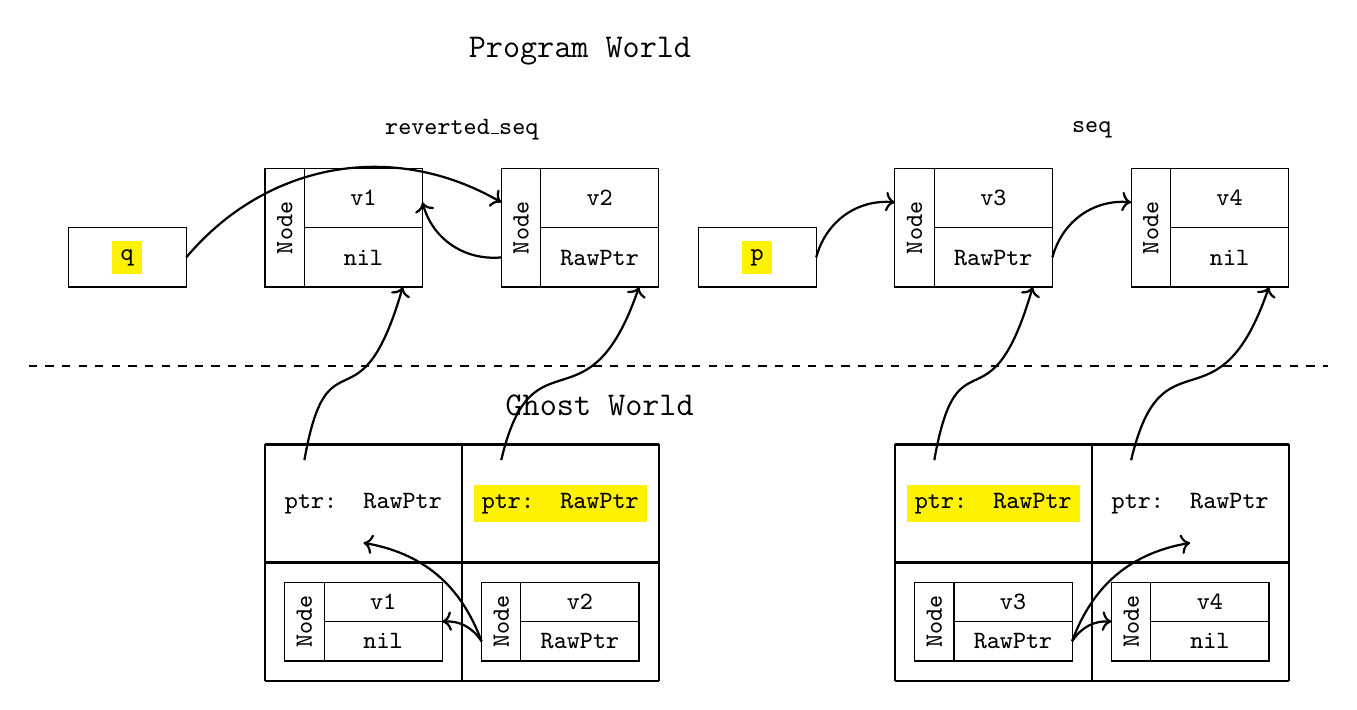
\begin{tikzpicture}
    \node[font=\large\bfseries] at (4,7.5) {\texttt{Program World}};
   
    \node[font=\small\bfseries] at (2.5,6.5) {\texttt{reverted\_seq}};
        
    % Head pointer now points to v2 (the new head after reversal)
    \draw (-2.5,4.5) rectangle (-1,5.25);
    \node[font=\small] at (-1.75,4.875) {\texttt{\colorbox{yellow}{q}}};
    \draw[->, thick, bend left=40] (-1,4.875) to (3,5.575);
    
    % First Node (v1) - now the tail
    \draw (0,4.5) rectangle (0.5,6);
    \draw (0.5,4.5) rectangle (2,5.25);
    \draw (0.5,5.25) rectangle (2,6);
    \node[rotate=90, font=\small] at (0.25,5.25) {\texttt{Node}};
    \node[font=\small] at (1.25,5.625) {\texttt{v1}};
    \node[font=\small] at (1.25,4.875) {\texttt{nil}};
    
    % Reversed arrow: v2 now points to v1
    \draw[->, thick, bend left=40] (3,4.875) to (2,5.575);
    
    % Second Node (v2) - now the head
    \draw (3,4.5) rectangle (3.5,6);
    \draw (3.5,4.5) rectangle (5,5.25);
    \draw (3.5,5.25) rectangle (5,6);
    \node[rotate=90, font=\small] at (3.25,5.25) {\texttt{Node}};
    \node[font=\small] at (4.25,5.625) {\texttt{v2}};
    \node[font=\small] at (4.25,4.875) {\texttt{RawPtr}};
    
    % Dashed divider line
    \draw[dashed, thick] (-3,3.5) -- (5.5,3.5);
    
    
    % Manual grid lines for 2 columns
    % Vertical lines
    \draw[black, thick] (0,-0.5) -- (0,2.5);
    \draw[black, thick] (2.5,-0.5) -- (2.5,2.5);
    \draw[black, thick] (5,-0.5) -- (5,2.5);
    
    % Horizontal lines
    \draw[black, thick] (0,-0.5) -- (5,-0.5);     % Bottom
    \draw[black, thick] (0,1) -- (5,1);          % Middle
    \draw[black, thick] (0,2.5) -- (5,2.5);      % Top
    
    % Column 1 (v1) - now points to nil
    \node[font=\small] at (1.25,1.75) {\texttt{ptr: RawPtr}};
    \draw (0.25,-0.25) rectangle (0.75,0.75);
    \draw (0.75,-0.25) rectangle (2.25,0.25);
    \draw (0.75,0.25) rectangle (2.25,0.75);
    \node[rotate=90, font=\small] at (0.5,0.25) {\texttt{Node}};
    \node[font=\small] at (1.5,0.5) {\texttt{v1}};
    \node[font=\small] at (1.5,0) {\texttt{nil}};
    
    % Column 2 (v2) - now points to v1
    \node[font=\small] at (3.75,1.75) {\texttt{\colorbox{yellow}{ptr: RawPtr}}};
    \draw (2.75,-0.25) rectangle (3.25,0.75);
    \draw (3.25,-0.25) rectangle (4.75,0.25);
    \draw (3.25,0.25) rectangle (4.75,0.75);
    \node[rotate=90, font=\small] at (3,0.25) {\texttt{Node}};
    \node[font=\small] at (4,0.5) {\texttt{v2}};
    \node[font=\small] at (4,0) {\texttt{RawPtr}};
    
    % Cross-reference arrows from Ghost World to Program World
    \draw[->, thick] (0.5,2.3) .. controls (0.8,4) and (1.2,2.6) .. (1.75,4.5);
    \draw[->, thick] (3,2.3) .. controls (3.4,4) and (4.1,2.6) .. (4.75,4.5);
    
    % Internal Ghost World arrows - reversed direction
    \draw[->, thick, bend right=30] (2.75,0) to (2.25,0.25);
    \draw[->, thick, bend right=30] (2.75,0) to (1.25,1.25);
    
    
    % ============== SCHEME 3: Second half (v3 -> v4) ==============
    \node[font=\small\bfseries] at (10.5,6.5) {\texttt{seq}};
    
    \draw (5.5,4.5) rectangle (7,5.25);
    \node[font=\small] at (6.25,4.875) {\texttt{\colorbox{yellow}{p}}};
    \draw[->, thick, bend left=40] (7,4.875) to (8,5.575);
    
    % Third Node
    \draw (8,4.5) rectangle (8.5,6);
    \draw (8.5,4.5) rectangle (10,5.25);
    \draw (8.5,5.25) rectangle (10,6);
    \node[rotate=90, font=\small] at (8.25,5.25) {\texttt{Node}};
    \node[font=\small] at (9.25,5.625) {\texttt{v3}};
    \node[font=\small] at (9.25,4.875) {\texttt{RawPtr}};
    
    % Arrow to fourth node
    \draw[->, thick, bend left=40] (10,4.875) to (11,5.575);
    
    % Fourth Node
    \draw (11,4.5) rectangle (11.5,6);
    \draw (11.5,4.5) rectangle (13,5.25);
    \draw (11.5,5.25) rectangle (13,6);
    \node[rotate=90, font=\small] at (11.25,5.25) {\texttt{Node}};
    \node[font=\small] at (12.25,5.625) {\texttt{v4}};
    \node[font=\small] at (12.25,4.875) {\texttt{nil}};
    
    % Dashed divider line
    \draw[dashed, thick] (5,3.5) -- (13.5,3.5);
    
    % Ghost World
    \node[font=\large\bfseries] at (4.25,3) {\texttt{Ghost World}};
    
    % Manual grid lines for 2 columns
    % Vertical lines
    \draw[black, thick] (8,-0.5) -- (8,2.5);
    \draw[black, thick] (10.5,-0.5) -- (10.5,2.5);
    \draw[black, thick] (13,-0.5) -- (13,2.5);
    
    % Horizontal lines
    \draw[black, thick] (8,-0.5) -- (13,-0.5);     % Bottom
    \draw[black, thick] (8,1) -- (13,1);          % Middle
    \draw[black, thick] (8,2.5) -- (13,2.5);      % Top
    
    % Column 1
    \node[font=\small] at (9.25,1.75) {\texttt{\colorbox{yellow}{ptr: RawPtr}}};
    \draw (8.25,-0.25) rectangle (8.75,0.75);
    \draw (8.75,-0.25) rectangle (10.25,0.25);
    \draw (8.75,0.25) rectangle (10.25,0.75);
    \node[rotate=90, font=\small] at (8.5,0.25) {\texttt{Node}};
    \node[font=\small] at (9.5,0.5) {\texttt{v3}};
    \node[font=\small] at (9.5,0) {\texttt{RawPtr}};
    
    % Column 2
    \node[font=\small] at (11.75,1.75) {\texttt{ptr: RawPtr}};
    \draw (10.75,-0.25) rectangle (11.25,0.75);
    \draw (11.25,-0.25) rectangle (12.75,0.25);
    \draw (11.25,0.25) rectangle (12.75,0.75);
    \node[rotate=90, font=\small] at (11,0.25) {\texttt{Node}};
    \node[font=\small] at (12,0.5) {\texttt{v4}};
    \node[font=\small] at (12,0) {\texttt{nil}};
    
    % Cross-reference arrows from Ghost World to Program World
    \draw[->, thick] (8.5,2.3) .. controls (8.8,4) and (9.2,2.6) .. (9.75,4.5);
    \draw[->, thick] (11,2.3) .. controls (11.4,4) and (12.1,2.6) .. (12.75,4.5);
    
    % Internal Ghost World arrows
    \draw[->, thick, bend left=30] (10.25,0) to (10.75,0.25);
    \draw[->, thick, bend left=30] (10.25,0) to (11.75,1.25);
    
    
    
\end{tikzpicture}
    
    \caption{Memory representation of data mid-execution.}
    \label{fig:invariant}
  \end{figure} 
    In order to ensure the post-conditions, we need to maintain during the loop that the pointer \texttt{q} and the sequence \texttt{reverted\_seq} form a valid list, the latter will hold, at the end of the program, the sequence corresponding to the reversed list. This invariant is crucial to guarantee the first post-condition at the end of the iteration.
    \begin{minted}{rust}
         #[invariant(Self::list(q, *reverted_seq))]
    \end{minted}
    
    We must also ensure that the remaining part of the list, represented by the pointer \texttt{p} and the sequence \texttt{seq}, continues to form a valid list. 
    \begin{minted}{rust}
         #[invariant(Self::list(p, **seq))]
    \end{minted}
    More importantly, we use the predicate \texttt{inverse} to check that the elements in \texttt{reverted\_seq} are pushed in the reverse order. Otherwise, if we relied on a built-in reversal function, the correctness would not be guaranteed, as illustrated in \autoref{fig:invariant}.
     \begin{minted}[breaklines=true]{rust}
      #[invariant(Self::inverse(_seq0.subsequence(0, reverted_seq.len()), *reverted_seq, 0, reverted_seq.len()))]
     \end{minted}
    
    
\end{itemize}
\section{Conclusion and perspectives}
\subsection{\scol{Conclusion}}
This work successfully addresses the challenge of formally verifying in-place linked list reversal in the presence of shared data structures using \creusot{}. I have learned many concepts through this research work, not only about formal verification but also about program semantics and notions about the provers' compilers.

\subsection{\scol{Perspectives}}
we are looking forward to extending the proof to lasso structures and, more importantly, to proving the Morris~\cite{morris} tree traversal algorithm, which was my initial subject. Unfortunately, due to the complexity of the proof compared to the given time, We decided to work on a simpler but very important algorithm, which is the list reversal.
\newpage
\printbibliography

\newpage

\section{Appendix}

\hypertarget{reversal}{\subsection{\scol{\texttt{in\_place\_reversal} algorithm}}}
\begin{align*}
&\texttt{j := nil; while i } \texttt{<>} \texttt{ nil do} \\
&\quad \quad \texttt{(k := [i + 1]; [i + 1] := j; j := i; i := k).}
\end{align*}
\subsection{\scol{Code}}
\begin{minted}[breaklines=true]{rust}
extern crate creusot_contracts;
use ::std::ptr;
use creusot_contracts::ptr_own::{PtrOwn, RawPtr};
use creusot_contracts::*;
pub struct Node<T> {
    elem: T,
    pub next: RawPtr<Node<T>>,
}

impl<T> Node<T> {
    #[predicate]
    #[variant(perm_seq.len())]
    fn list(l: RawPtr<Self>, perm_seq: Seq<PtrOwn<Node<T>>>) -> bool {
        pearlite! {
            if l.is_null_logic() {
                perm_seq.len() == 0
            } else {
                 if perm_seq.len() > 0 {
                    let ptr = perm_seq[0].ptr();
                    l == ptr && Self::list(perm_seq[0].val().next, perm_seq.tail())
                } else {
                    false
                }
            }
        }
    }

    #[ensures(Self::list(result.0, *result.1))]
    #[ensures(result.0.is_null_logic())]
    pub fn empty() -> (RawPtr<Self>, Ghost<Seq<PtrOwn<Node<T>>>>) {
        (ptr::null(), Seq::new())
    }

    #[requires(Self::list(l, **seq))]
    #[ensures(Self::list(result,  *^seq))]
    #[ensures(forall<i:Int> 0 <= i && i < (^seq).tail().len() ==> seq[i] == (^seq).tail()[i])]
    #[ensures((^seq)[0].val().elem == e)]
    #[ensures((^seq)[0].ptr() == result)]
    #[ensures((^seq).len() == seq.len() + 1)]
    pub fn cons(e: T, l: RawPtr<Self>, seq: &mut Ghost<Seq<PtrOwn<Node<T>>>>) -> RawPtr<Self> {
        let (raw, own) = PtrOwn::new(Node { elem: e, next: l });

        let _seq2 = snapshot!(**seq);
        ghost!(seq.push_front_ghost(own.into_inner()));
        proof_assert!(*_seq2 == seq.tail());

        raw
    }

    #[requires(Self::list(p, **seq))]
    #[requires(0 <= nth@ && nth@ < seq.len() )]
    #[ensures(seq[nth@].val().elem == *result)]
    pub fn nth(mut p: RawPtr<Self>, nth: i128, seq: &Ghost<Seq<PtrOwn<Node<T>>>>) -> &T {
        let mut i = 0;
        proof_assert!(**seq == seq.subsequence(0, seq.len()));
        #[invariant(0 <= i@ && i@ <= nth@)]
        #[invariant(Self::list(p, seq.subsequence(i@, seq.len())))]
        loop {
            let rw = unsafe {
                PtrOwn::as_ref(p, ghost!(seq.get_ghost(Int::new(i).into_inner()).unwrap()))
            };

            if i == nth {
                return &rw.elem;
            }

            p = rw.next;
            proof_assert!(seq.subsequence(i@, seq.len()).tail() == seq.subsequence(i@+1, seq.len()));
            i += 1;
        }
    }

    #[predicate]
    pub fn inverse(seq: Seq<PtrOwn<Node<T>>>, other: Seq<PtrOwn<Node<T>>>, lb: Int, lh: Int) -> bool
    where
        T: Sized,
    {
        pearlite! {
             forall<i: Int>
            lb <= i && i < lh
            ==> seq[i].val().elem == other[other.len() - i - 1].val().elem
        }
    }

    #[requires(Self::list(p, **seq))]
    #[ensures(Self::list(result, *^seq))]
    #[ensures(seq.len() == (^seq).len())]
    #[ensures(Self::inverse(**seq, *^seq, 0, (*^seq).len()))]
    pub fn reverse_in_place(
        mut p: RawPtr<Self>,
        seq: &mut Ghost<Seq<PtrOwn<Node<T>>>>,
    ) -> RawPtr<Self> {
        snapshot! {
            let _ = Seq::<T>::ext_eq;
        };
        let mut q: *const Node<T> = ptr::null();
        let mut reverted_seq = Seq::new();
        let _seq0 = snapshot!(**seq);

        #[invariant(Self::list(q, *reverted_seq))]
        #[invariant(Self::list(p, **seq))]
        #[invariant(Self::inverse(_seq0.subsequence(0, reverted_seq.len()), *reverted_seq, 0, reverted_seq.len()))]
        #[invariant(reverted_seq.len() + seq.len() == _seq0.len())]
        #[invariant(**seq == _seq0.subsequence(reverted_seq.len(), _seq0.len()))]
        #[invariant(inv(seq))]
        #[invariant(inv(reverted_seq))]
        while !p.is_null() {
            let _sloop_entry = snapshot!(**seq);
            let _revs_loop_entry = snapshot!(*reverted_seq);
            let p2 =
                unsafe { PtrOwn::as_mut(p, ghost!(seq.get_mut_ghost(*ghost!(0int)).unwrap())) };
            let next = p2.next;
            p2.next = q;
            q = p;
            p = next;
            let _sloop_exit = snapshot!(**seq);

            ghost!((*reverted_seq).push_front_ghost(seq.pop_front_ghost().unwrap()));

            //a0156: Assertion used to prove invariant #1 (we can remove it and use use_th seq.FreeMonoid instead)
            proof_assert!(reverted_seq.tail() == *_revs_loop_entry);

            //Hypothesis: invariant(Self::list (p, **seq))
            // We need to add to the hypothesis the fac that the tail of the previous seq is the new seq
            //a1369
            proof_assert!((*_sloop_exit).tail() == **seq);

            //In order to proof the last assertion, we need the following assertion
            //It esnures that seq.tail() didn't change between the beginig of the loop and the end, what ensures the stability of our invariant
            //a7070
            proof_assert!((*_sloop_exit).tail() == (*_sloop_entry).tail());

            //this should be enough to prove #[invariant(Self::list (p, **seq))], whith using the latter, creusot proves well the remaining invariant about q
            //proof_assert!(Self::list(p, (*snap2).tail()));
            //a1313
            proof_assert!(Self::list(p, (*_sloop_exit).tail()));
            // ==> invariant #1 checks for iteration n+1
        }
        //Pour montrer ensures#1 (ensures(seq.len() == (^seq).len() && Self::inverse(**seq, *^seq, 0, seq.len())))
        //a4224
        proof_assert!(_seq0.subsequence(0, reverted_seq.len()) == *_seq0);
        ghost!(**seq = reverted_seq.into_inner());
        q
    }
}

#[ensures(Node::list(result.0, *result.1))]
#[ensures(result.1.len() == vec.view().len())]
#[ensures(forall<i: Int> 0 <= i && i < vec.view().len() ==> (*result.1)[i].val().elem == vec.view()[i])]
pub fn list_of_vector1<T>(mut vec: Vec<T>) -> (RawPtr<Node<T>>, Ghost<Seq<PtrOwn<Node<T>>>>) {
    //Takes possession of elements in the vector
    let (mut l, mut seq) = Node::empty();
    let _vec0 = snapshot!(vec);
    #[invariant(forall<i: Int>
        vec.view().len() <= i && i < _vec0.view().len() ==> seq[i - vec.view().len()].val().elem == _vec0.view()[i])]
    #[invariant(Node::list(l, *seq))]
    #[invariant(vec.view().len() + seq.len() == _vec0.view().len())]
    #[invariant(forall<i: Int> 0 <= i && i < vec.view().len() ==> vec.view()[i] == _vec0.view()[i])]
    #[invariant(inv(seq))]
    loop {
        if let Some(v) = vec.pop() {
            l = Node::cons(v, l, &mut seq);
        } else {
            break;
        }
    }
    (l, seq)
}

pub fn tr() {
    let v1 = creusot_contracts::vec![1, 5, 3];
    let (list1, mut _seq1) = list_of_vector1(v1.clone());
    assert!(*Node::nth(list1, 0, &_seq1) == 1);
    assert!(*Node::nth(list1, 1, &_seq1) == 5);
    assert!(*Node::nth(list1, 2, &_seq1) == 3);
    let l2 = Node::reverse_in_place(list1, &mut _seq1);
    assert!(*Node::nth(l2, 2, &_seq1) == 1);
    assert!(*Node::nth(l2, 1, &_seq1) == 5);
    assert!(*Node::nth(l2, 0, &_seq1) == 3);

    print!("ok");
}
\end{minted}


\end{document}
